\documentclass{article}
\usepackage{amsfonts, amsmath, amssymb, amsthm} % Math notations imported
\usepackage{enumitem}
\usepackage{graphicx}
\usepackage{tabularx}
\usepackage[margin=1in]{geometry}
\usepackage{setspace}
\graphicspath{{./images/}} % Path to images

% \begin{figure}[htb!]
%      \centering
%      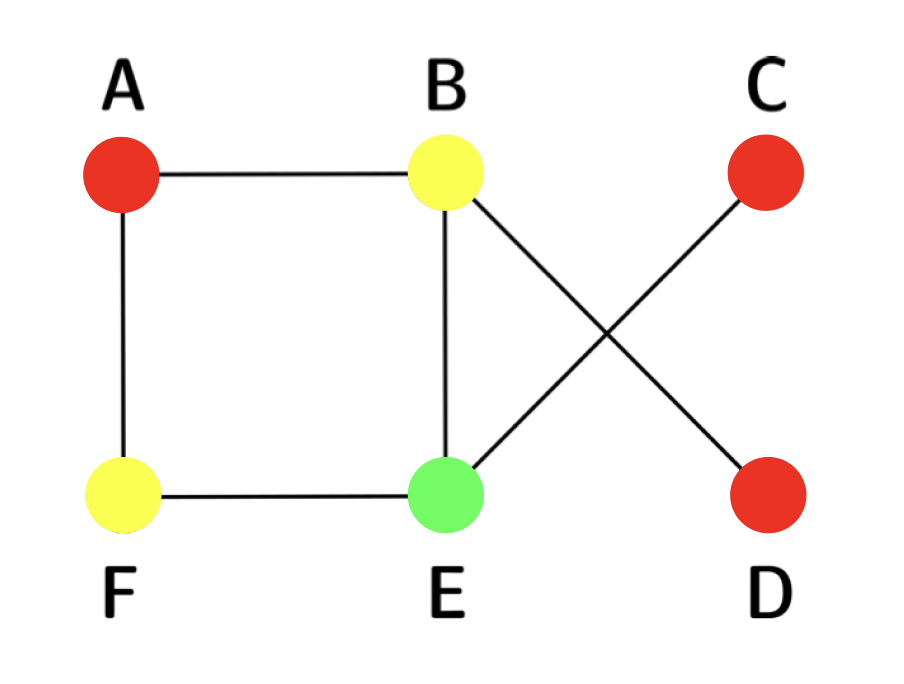
\includegraphics[scale=0.5]{coloring.png}
%      \caption{Coloring of the graph.}
% \end{figure}

% \begin{figure}[htb]
%     \qquad
%     \begin{minipage}{.4\textwidth}
%         \centering
%         {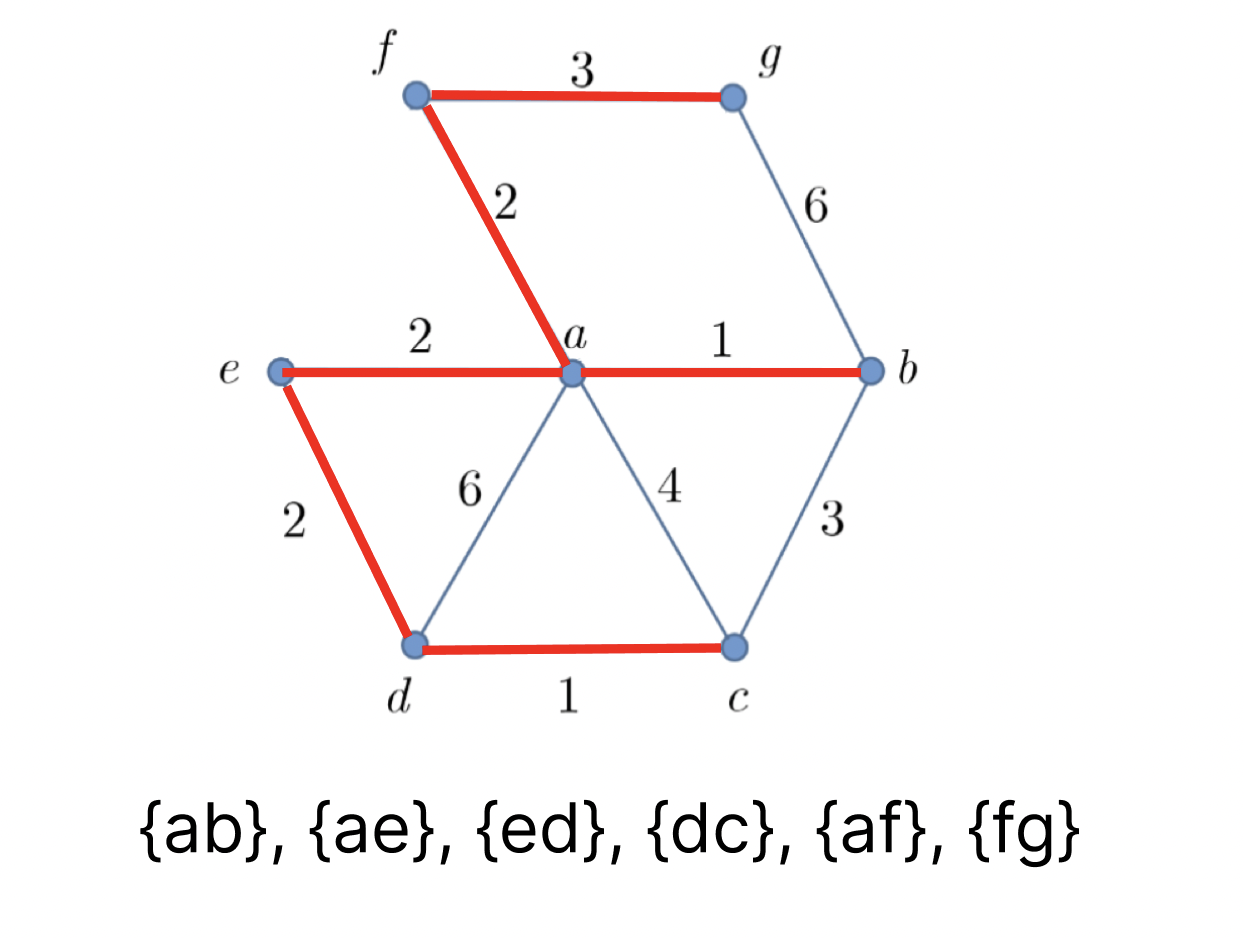
\includegraphics[scale=0.35]{prims.png}}
%         \qquad\qquad\emph{Prim's}\label{fig:1}
%     \end{minipage}    
%     \qquad
%     \begin{minipage}{.4\textwidth}
%         \centering
%         {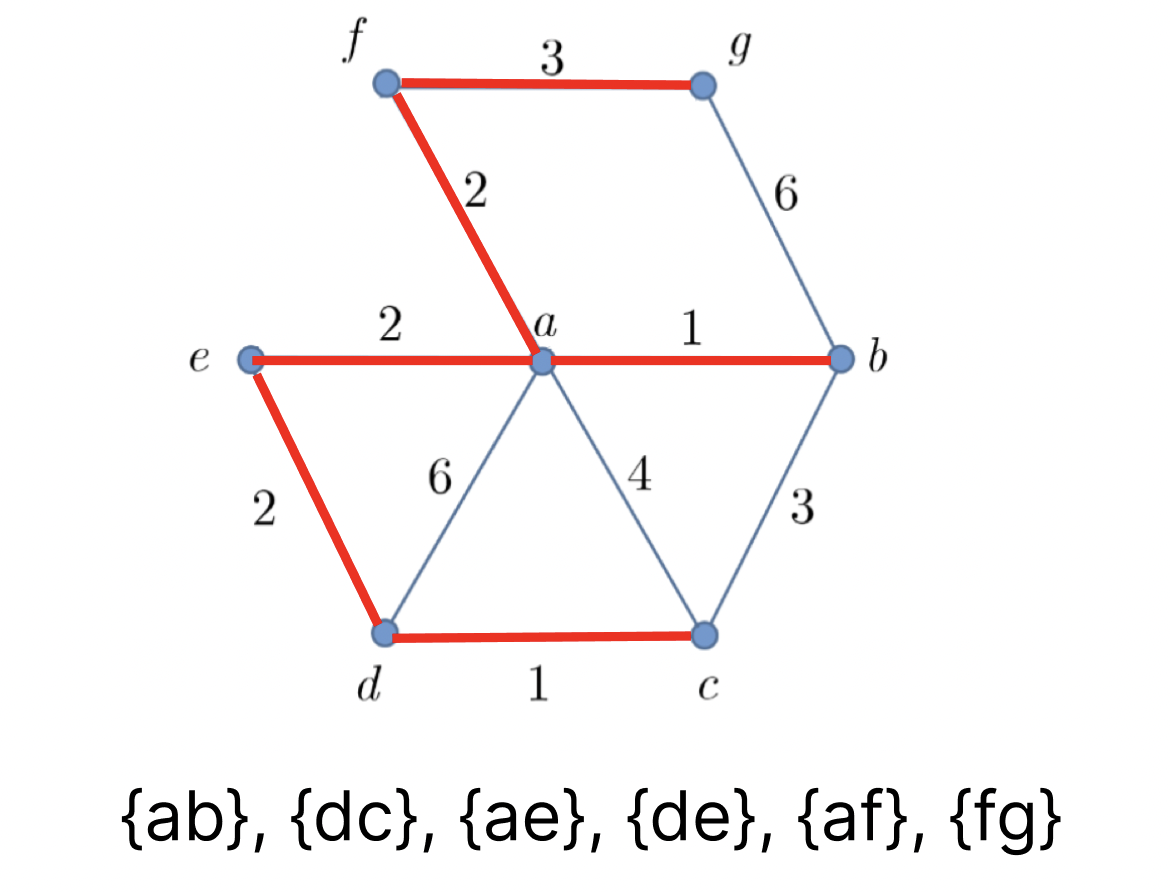
\includegraphics[scale=0.35]{kruskal.png}}
%         \qquad\qquad\emph{Kruskal's}\label{fig:2}
%     \end{minipage}        
% \end{figure} 

\newtheorem{thm}{Theorem}
\newtheorem{proposition}[thm]{Proposition}
\newtheorem{cor}[thm]{Corollary}

% title information
\title{Math 128A HW1}
\author{Neo Lee}
\date{09/06/2023}

\setstretch{1.15}
% main content
\begin{document} 

% placing title information; comment out if using fancyhdr
\maketitle 

\section*{Section 1.1}
\subsection*{Problem 2c}
\begin{proposition}
    $f(x) = -3\cdot tan(2x) + x = 0$ has at least one solution for $x \in [0,1]$.
\end{proposition}
\begin{proof}
    Note that the interval is end point inclusive. 
    We have $f(0) = 0$, which is immediately one solution to the equation.
\end{proof}

\subsection*{Problem 2d}
\begin{proposition}
    $f(x) = ln(x)-x^2+\frac{5}{2}x - 1 = 0$ has at least one solution for $x \in [\frac{1}{2},1]$.
\end{proposition}
\begin{proof}
    $f(\frac{1}{2}) \approx -0.693, f(1) = 0.5$. Hence, by the intermediate value theorem, there 
    exists a solution in the interval.
\end{proof}

\subsection*{Problem 4d}
Find interval containing solutions to $x^3 + 4.001x^2 + 4.002x + 1.101 = 0$.
\begin{proof}[Solution]
    Since there is no further intructions on the error bound of the interval, we will proceed with 
    the simplest calculus method by finding critical points. Consider the first derivative and set 
    it equal to zero.
    \begin{align*}
        3x^2 + 8.002x + 4.002 & = 0 \\
        x & = \frac{-8.002 \pm \sqrt{8.002^2 - 4\cdot 3\cdot 4.002}}{2\cdot 3} \\
        & \approx \frac{-8 \pm 4}{6} = \frac{-4 \pm 2}{3}.
    \end{align*}

    Now, we can look at both points respectively. $f(-2) = 1.101, f(\frac{-2}{3}) \approx -0.0851$.
    By intermediate theorem, we know that there exists a solution in $[-2, \frac{-2}{3}]$. Now, by 
    simple observation, we can easily conclude that the equation tends to $-\infty$ when $x 
    \rightarrow -\infty$ and tends to $\infty$ when $x \rightarrow \infty$. Hence, by intermediate 
    theorem, there exists one solution in $[-\infty, -2]$ and one in $[\frac{-2}{3}, \infty]$.
\end{proof}

\subsection*{Problem 6a}
Find $max_{a\le x\le b}|f(x)|$ for $f(x) = \frac{2x}{x^2+1}$ on $[0,2]$.
\begin{proof}[Solution]
    We proceed by finding the critical points of $f(x)$ on $[0,2]$.

    \begin{align*}
        f'(x) & = \frac{2(x^2+1) - 2x(2x)}{(x^2+1)^2} \\
              & = \frac{2 - 2x^2}{(x^2+1)^2} \\
              & = 0 \text{ when } x = \pm 1.
    \end{align*}

    Then, we have $f(0) = 0, f(1) = 1, f(2) = \frac{4}{5}$. Hence, the maximum value of $f(x)$ on 
    $[0,2]$ is $1$ when $x=1$.
\end{proof}

\subsection*{Problem 14}
Let $f(x) = 2x\cdot cos(2x) - (x-2)^2$ and $x_0 = 0$.
\begin{enumerate}[label=(\alph*)]
    \item Find the third Taylor polynomial $P_3(x)$ and use it to approximate $f(0.4)$.
    \begin{proof}[Solution]
        \begin{align*}
            f'(x) & = 2cos(2x) - 4xsin(2x) - 2(x-2), \\
            f''(x) & = -8sin(2x) - 8xcos(2x) - 2 \\
            f'''(x) & = 16xsin(2x) - 24cos(2x).
        \end{align*}

        Now, we have $f(0) = -4, f'(0) = 6, f''(0) = -2, f'''(0) = -24$. Hence, the third Taylor 
        polynomial $P_3(x) = -4 + 6x -x^2 -4x^3$, and $f(0.4) \approx -2.016$.
    \end{proof}

    \item Use the error formula in Taylor's Theorem to find an upper bound for the error 
    $|f(0.4) - P_3(0.4)|$

    \begin{proof}[Solution]
        \begin{align*}
            f^4(x) & = 64sin(2x) + 32xcos(2x) \\
            R_3(x) & = \frac{f^4(\xi(x))}{4!}(0.4)^4 \qquad \emph{for } 0 \le \xi(x) \le 0.4.
        \end{align*}

        Hence, \begin{align*}
            |f(0.4) - P_3(0.4)| = |R_3(0.4)| & = \frac{f^4(\xi(x))}{4!}(0.4)^4 \\
            & = \frac{64sin(2\xi(x))+32\cdot \xi(x)cos(2\xi(x))}{24}\times 0.0256 \\
            & \le \frac{64+32\cdot \xi(x)}{24}\times 0.0256 \qquad (\emph{notice } 0 \le sin(2\xi(x)),
            cos(2\xi(x))\le 1)\\
            & \le \frac{64 + 32\times 0.4}{24}\times 0.0256 \\
            & \le 0.08192.
        \end{align*}
    \end{proof}

    \item Find the third Taylor polynomial $P_4(x)$ and use it to approximate $f(0.4)$.
    \begin{proof}[Solution]
        \begin{align*}
            f^4(x) & = 64sin(2x) + 32xcos(2x) \\
            f^4(0) & = 0 \\
            P_4(x) & = -4 + 6x -x^2 \\
            f(0.4) & \approx P_4(0.4) = -2.016.
        \end{align*}
    \end{proof}

    \item Use the error formula in Taylor's Theorem to find an upper bound for the error
    $|f(0.4) - P_4(0.4)|$. Compute the actual error.

    \begin{proof}[Solution]
        \begin{align*}
            f^5(x) & = 160cos(2x) - 64xsin(2x) \\
            |f(0.4) - P_4(0.4)| = |R_4(x)| & = \frac{f^5(\xi(x))}{5!}(0.4)^5 \qquad 
            \emph{for } 0 \le \xi(x) \le 0.4. \\
            & \le \frac{160}{5!}\times 0.4^5 \\
            & \le 0.01366.
        \end{align*}
    \end{proof}
\end{enumerate}

\subsection*{Problem 26} 

\begin{enumerate}[label=\alph*.]
    \item Use Rolle's Theorem to show that $f'(z_i) = 0$ for $n$ numbers in $[a,b]$ with 
    $a < z_1 < z_2 < \cdots < z_{n} < b$.

    \begin{proof}[Solution]
        We are unable to show that without further assumption. Since our goal is proving the 
        Generalized Rolle's Theorem, we will proceed with the assumption that $f(x)$ is $n$ times 
        differentiable on $(a, b)$, and that $f(x) = f(a) = f(b)$ at $n - 1$ distinct numbers such 
        that $a < x_2 < x_3 \cdots < x_n < b$. For clarity, we will also denote $x_1 = a$ and 
        $x_{n+1} = b$ such that $a = x_1 < x_2 < \cdots < x_{n+1} = b$.

        Now consider each interval $[x_i, x_{i+1}]$ for all $i\in [0, 1, \dots, n]$. Notice that 
        there are $n$ such intervals and $f(x_i) = f(x_{i+1})$. Hence, by 
        Rolle's Theorem, there exists $z_i \in (x_i, x_{i+1})$ such that $f'(z_i) = 0$. Therefore, 
        we can conclude that $f'(z_i) = 0$ for $n$ numbers in $[a,b]$ with $a < z_1 < z_2 < \cdots 
        < z_{n} < b$.
    \end{proof}
    
    \item Use Rolle's Theorem to show that $f''(w_i) = 0$ for $n-1$ numbers in $[a,b]$ with 
    $z_1 < w_1 < z_2 < w_2 \cdots w_{n} < z_{n} < b$.

    \begin{proof}[Solution]
        We have shown from (a) that $f'(z_i) = 0$ for $i \in [1, 2, \dots, n]$. Now consider each 
        interval $(z_i, z_{i+1})$ for $i \in [1, 2, \dots, n-1]$. There are $n-1$ such intervals and 
        $f'(z_i) = f'(z_{i+1})$. Hence, by Rolle's Theorem, there exists $w_i \in (z_i, z_{i+1})$ 
        such that $f''(w_i) = 0$. Therefore, we can conclude that $f''(w_i) = 0$ for $n-1$ numbers 
        in $[a,b]$ with $a < z_1 < w_1 < z_2 < w_2 \cdots w_{n-1} < z_{n} < b$.
    \end{proof}

    \item Continue the arguments in parts (a) and (b) to show that for each $j = 1, 2, \dots, n$, 
    there are $n+1-j$ distinct numbers in $[a,b]$, where $f^{(j)}$ is 0.

    \begin{proof}[Solution]
        We can easily show by induction on $j$. Base case is already established in (a). Now, assume that 
        $f^{(k)}(y_i) = 0$ for $n+1-k$ distinct numbers in $[a,b]$. Consider each interval $(y_i, 
        y_{i+1})$ for $i\in [1, 2, \dots, n-k]$. There are $n-k$ such intervals and $f^{(k)}(y_i) =
        f^{(k)}(y_{i+1})$. Hence, by Rolle's Theorem, there exists $n-k$ numbers of $u_i \in (y_i, y_{i+1})$ such 
        that $f^{(k+1)}(u_i) = 0$. Therefore, we can conclude that $f^{(k+1)}(u_i) = 0$ for $n-k = 
        n + 1 - (k+1)$ distinct numbers in $[a,b]$. 

        Hence, by induction, we can conclude that for each $j = 1, 2, \dots, n$, there are $n+1-j$
        distinct numbers in $[a,b]$, where $f^{(j)}$ is 0.
    \end{proof}

    \item  Show that part (c) implies the conclusion of the Generalized Rolle's Theorem.
    
    \begin{proof}[Solution]
        Notice our only assumptions are that $f(x)$ is $n$ times differentiable on $(a, b)$, and that 
        $f(x) = f(a) = f(b)$ at $n - 1$ distinct numbers such that $a < x_2 < x_3 \cdots < x_n < b$, 
        which is equivalent to saying $f(x)$ is constant for $n+1$ distinct numbers in $[a,b]$. 

        With the mentioned assumptions, we concluded that there are $n+1-j$ distinct numbers in 
        $[a,b]$, where $f^{(j)}$ is 0. Now take $j = n$, we have $n+1-n = 1$ distinct number in 
        $[a,b]$, where $f^{(n)}$ is 0. Hence, we can conclude that there exists $c \in (a,b)$ such 
        that $f^{(n)}(c) = 0$.

        Notice this is exactly what the Generalized Rolle's Theorem says.
    \end{proof}


\end{enumerate}

\section*{Section 1.2}
\subsection*{Problem 2c}
Compute the absolute error and relative error in approximations of $p$ by $p^*$: $p = 8!, p^* = 
39900$.

\begin{proof}[Solution]
    \begin{align*}
        |p - p^*| & = 8! - 39900 = 40320 - 39900 = 420. \\
        \frac{|p-p^*|}{p} & = \frac{420}{8!} =\frac{1}{96} \approx 0.0104.
    \end{align*}
\end{proof}

\subsection*{Problem 4b}
Find the largest interval in which $p^*$ must lie to approximate $p$ with relative error at most 
$10^{-4}$ for $p = e$.
\begin{proof}[Solution]
    \begin{align*}
        \frac{|p^*-e|}{e} & \le 10^{-4} \\
        |p^*-e| & \le 10^{-4}e \\
        |p^* - e| & \le 10^{-4}e \\
        (1-10^{-4})\cdot e & \le p^* \le (1+10^{-4})\cdot e \\
        0.9999\cdot e & \le p^* \le 1.0001\cdot e.
    \end{align*}

    If we want to find a numerical bound, we can arbitrarily choose $e = 2.71828$, the most commonly 
    used approximation of $e$. Then, we have 
    \begin{align*}
        2.71828\cdot 0.9999 & \le p^* \le 2.71828\cdot 1.0001 \\
        2.71800 & \le p^* \le 2.71855.
    \end{align*}

\end{proof}

\subsection*{Problem 12}
The number $e$ can be defined by $e = \sum^\infty_{n=0}(1/n!)$ where 
$n! = n(n-1)\cdots 2\cdot 1$
for $n\neq 0$ and $0! = 1$.
Compute the absolute error and relative error in the following approximations of $e$:
\begin{enumerate}[label=\alph*.]
    \item $\sum\limits^5_{n=0}\frac{1}{n!}$
    \begin{proof}[Solution]
        We will just plug in matlab and use the default $e$ value from matlab to compute the error.
        \begin{align*}
            |e - \sum\limits_{n=0}^{5}\frac{1}{n!}| & \approx 0.0016152 \\
            \frac{|e - \sum\limits_{n=0}^{5}\frac{1}{n!}|}{|e|} & \approx 0.00059418.
        \end{align*}
    \end{proof}
    
    \item $\sum\limits^{10}_{n=0}\frac{1}{n!}$
    \begin{proof}[Solution]
        We will just plug in matlab and use the default $e$ value from matlab to compute the error.
        \begin{align*}
            |e - \sum\limits_{n=0}^{10}\frac{1}{n!}| & \approx 2.7313 \times 10^{-8} \\
            \frac{|e - \sum\limits_{n=0}^{10}\frac{1}{n!}|}{|e|} & \approx 1.0048 \times 10^{-8}.
        \end{align*}
    \end{proof}
\end{enumerate}

\subsection*{Problem 22}
The Taylor polynomial of degree $n$ for $f(x) = e^x$ is $\sum_{i=0}^\infty(x^i/i!)$. Use the Taylor 
polynomial of degree nine and three-digit chopping arithmetic to find an approximation to $e^{-5}$ 
by each of the following methods.
\begin{enumerate}[label=\alph*.]
    \item $e^{-5} \approx \sum\limits_{i=0}^9\frac{(-5)^i}{i!} = 
    \sum\limits_{i=0}^9\frac{(-1)^i5^i}{i!}$.
    \begin{proof}[Solution]
        With three-digit chopping arithmetic, we have
        \begin{align*}
            \sum\limits_{i=0}^9\frac{(-1)^i5^i}{i!} & = 1 - 5 + \frac{25}{2} - \frac{125}{6} + 
            \frac{625}{24} - \frac{3120}{120} + \frac{15600}{720} - \frac{78000}{5040} + 
            \frac{390000}{40300} - \frac{1950000}{362000} \\
            & = 1 - 5 + 12.5 - 20.8 + 26.0 - 26.0 + 21.6 - 15.4 + 9.67 - 5.38 \\
            & = -1.81.
        \end{align*}
    \end{proof}
    
    \item $e^{-5} = \frac{1}{e^5} \approx \frac{1}{\sum_{i=0}^{9}\frac{5^i}{i!}}$.
    \begin{proof}[Solution]
        With three-digit chopping arithmetic, we have
        \begin{align*}
            \sum\limits_{i=0}^9\frac{(-1)^i5^i}{i!} & = 1 / \left(1 + 5 + \frac{25}{2} + \frac{125}{6} + 
            \frac{625}{24} + \frac{3120}{120} + \frac{15600}{720} + \frac{78000}{5040} + 
            \frac{390000}{40300} + \frac{1950000}{362000}\right) \\
            & = 1/ (1 + 5 + 12.5 + 20.8 + 26.0 + 26.0 + 21.6 + 15.4 + 9.67 + 5.38) \\
            & = 1/141 \\
            & = 0.00709.
        \end{align*}
    \end{proof}
    
    \item An approximate value of $e^{-5}$ correct to three digits is $6.74\times 10^{-3}$. 
    Which formula,(a) or (b), gives the most accuracy, and why?
    \begin{proof}[Solution]
        (b) obviously gives a more accurate answer. With (a) method, we are adding and subtracting 
        large numbers, which will cause a lot of cancellation and takes longer to converge. With 
        (b) method, we are only adding the numbers and taking the reciprocal. Dividing by an 
        increasing large number will cause the result to converge faster.
    \end{proof}
\end{enumerate}

\section*{Section 1.3}
\subsection*{Problem 8}
Suppose that $0 < q < p$ and that $\alpha_n = \alpha + O(n^{-p})$.
\begin{enumerate}[label=\alph*.]
    \item Show that $a_n = \alpha + O(n^{-q})$.
    \begin{proof}
        For $n \ge 1$,
        \begin{align*}
            \frac{n^q}{n^p} & \le 1 \\
            \frac{1}{n^p} & \le \frac{1}{n^q} \\
            n^{-p} & \le n^{-q} \\
            |a_n - \alpha| \le k\cdot n^{-p} & \le k\cdot n^{-q} \qquad
            (\emph{we know the existence of }k) \\
            |a_n -\alpha| & \le k\cdot n^{-q} \\
            a_n & = \alpha + O(n^{-q}).
        \end{align*}
    \end{proof}

    \item Make a table listing $1/n$, $1/n^2$, $1/n^3$, and $1/n^4$ for n = 5, 10, 100, and 1000 
    and discuss the varying rates of convergence of these sequences as $n$ becomes large.
    \begin{align*}
        \begin{tabularx}{0.8\textwidth} { 
            | >{\centering\arraybackslash}X 
            | >{\centering\arraybackslash}X 
            | >{\centering\arraybackslash}X 
            | >{\centering\arraybackslash}X 
            | >{\centering\arraybackslash}X | }
           \hline
           $n=$ & 5 & 10 & 100 & 1000 \\
           \hline
           $1/n$  & 0.2 & 0.1 & 0.01 & 0.001  \\
           \hline
           $1/n^2$  & 0.04  & 0.01 & 0.001 & 0.000001  \\
           \hline
           $1/n^3$  & 0.008  & 0.001 & $10^{-6}$ & $10^{-9}$  \\
           \hline
           $1/n^4$  & 0.0016  & 0.0001 & $10^{-8}$ & $10^{-12}$  \\
           \hline
        \end{tabularx}
    \end{align*}
    They all converge to 0, but at different rates. The value converges faster with a larger 
    exponent. For example, $1/n^4$ converges faster than $1/n^3$.
\end{enumerate}

\subsection*{Problem 15}
\begin{enumerate}[label=\alph*.]
    \item How many multiplications and additions are required to determine a sum of the form
    $$\sum_{i=1}^{n}\sum_{j=1}^{i}a_ib_j$$

    \begin{proof}[Solution]
        Let's expand the summation to count more easily.
        \begin{align*}
            \sum_{i=1}^{n}\sum_{j=1}^{i}a_ib_j = & a_1\cdot b_1 + (a_2\cdot b_1 + a_2\cdot b_2) + 
            (a_3\cdot b_1 + a_3\cdot b_2 + a_3\cdot b_3) \\ 
            & + \cdots + (a_n\cdot b_1 + a_n\cdot b_2 + \cdots + a_n\cdot b_n).
        \end{align*}
        Then, we can just count the number of $\cdot$ and $+$. The number of multiplication is 
        $1 + 2 + \cdots + n = \frac{n(n+1)}{2}$. The number of addition is $(n-1) + (n-1) + \cdots 
        + 1 = \frac{n(n-1)}{2} + (n-1)$. Hence, the total number of operations is $n^2+n-1$.
    \end{proof}

    \item Modify the sum in part (a) to an equivalent form that reduces the number of computations.
    \begin{proof}[Solution]
        \begin{align*}
            \sum_{i=1}^{n}\sum_{j=1}^{i}a_ib_j & = \sum_{i=1}^{n}a_i \cdot \left(\sum_{j=1}^{i}b_j\right).
        \end{align*}

        There are still $(n-1) + (n-1) + \cdots + 1 = \frac{n(n-1)}{2}+(n-1)$ additions. But the
        number of multiplication is reduced to $n$. Hence, the total number of operations is 
        $\frac{n(n-1)}{2} + (n-1) + n = \frac{n^2+3n-2}{2}$.
    \end{proof}
\end{enumerate}

\subsection*{Discussion Question 2 (p. 38)}
Construct an algorithm that has as input an integer $n \ge 1$,numbers $x_0,x_1,\dots,x_n$, and 
a number $x$ and that produces as output the product $(x-x_0)(x-x_1)\cdots(x-x_n)$.
\begin{proof}[Solution]
    \begin{align*}
        & \text{INPUT} \quad x_0, x_1, \dots, x_n, x \\
        & \text{OUTPUT} \quad \text{TOTAL} \\
        & \text{Step 1} \quad \text{Set } \text{TOTAL} = 1 \\
        & \text{Step 2} \quad \text{For } i = 0, 1, \dots, n \text{ do} \\
        & \qquad\qquad\qquad \text{Set TOTAL = TOTAL *} (x - x_i) \\
        & \text{Step 3} \quad \text{OUTPUT TOTAL;} \\
        & \qquad\qquad \text{STOP}
    \end{align*}
\end{proof}

\newpage
\section*{Section 2.1}
\subsection*{Problem 6d}
Use the Bisection method to find solutions, accurate to within $10^{-5}$ for 
\begin{align*}
    x+1-2sin(\pi x) = 0 \qquad (\emph{for $0\le x\le 0.5$ and $0.5 \le x \le 1$}).
\end{align*}
\begin{figure}[htb]
    \qquad
    \begin{minipage}{.4\textwidth}
        \centering
        {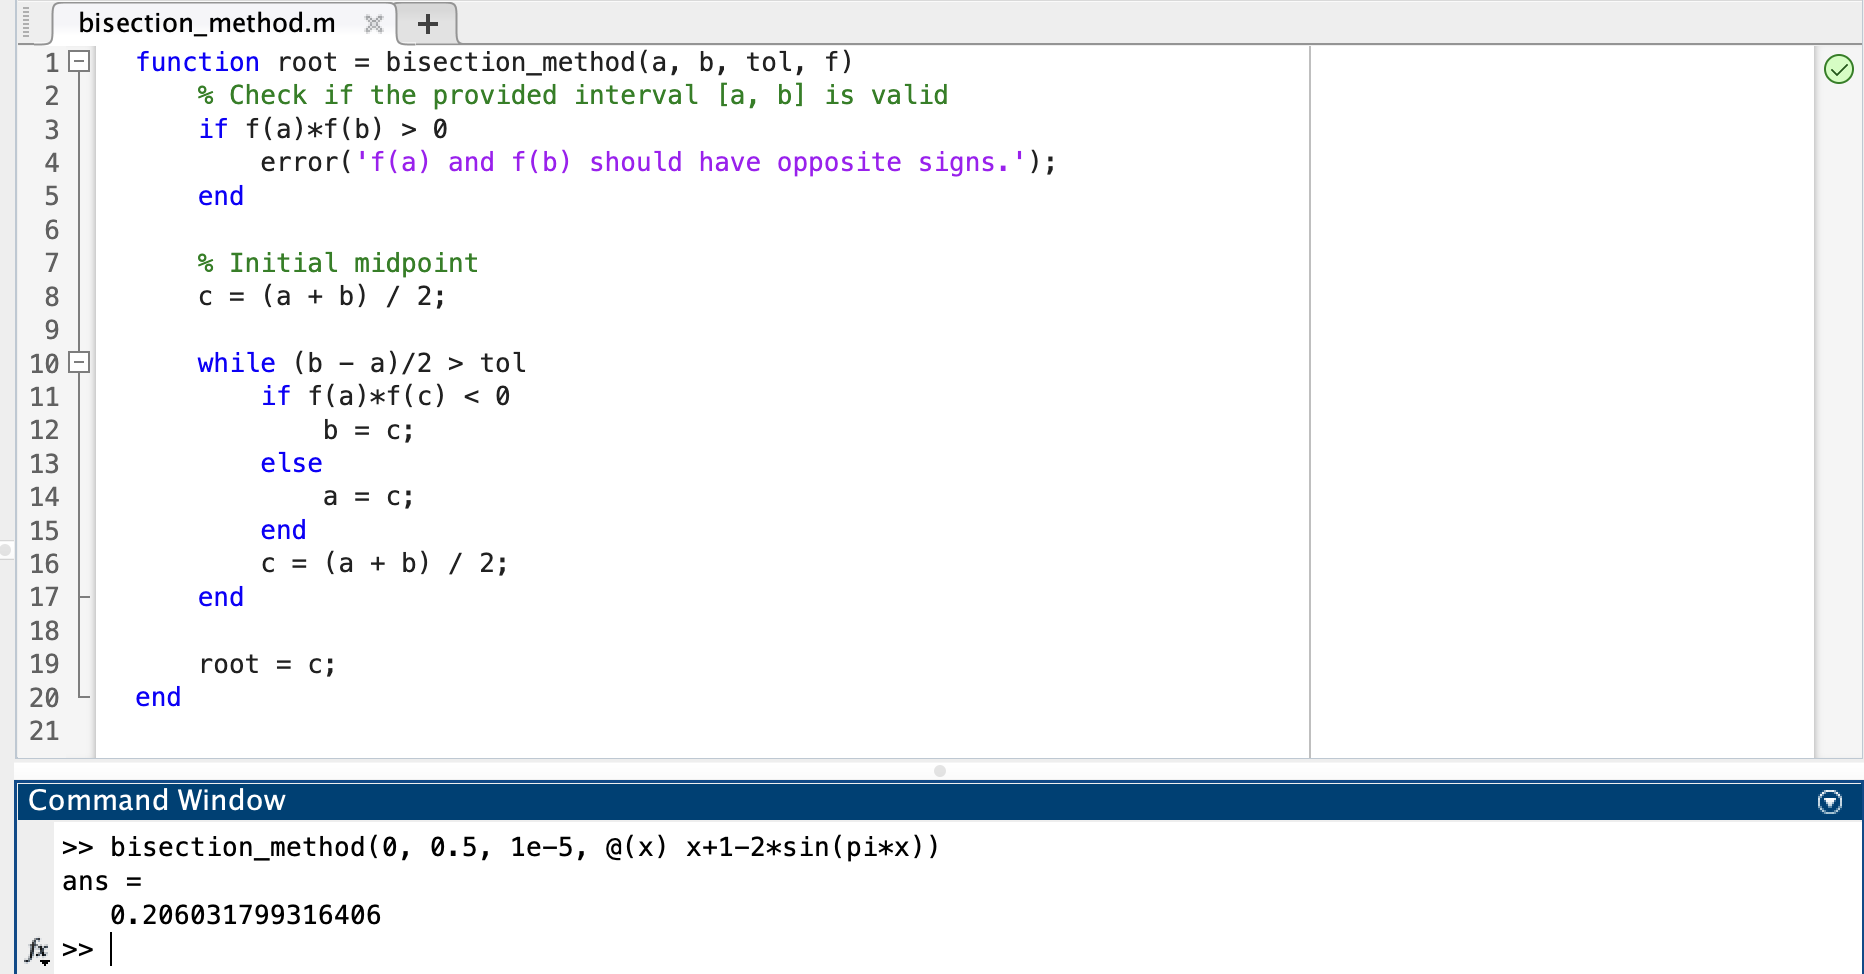
\includegraphics[scale=0.2]{first.png}}
        \qquad\qquad\emph{$0\le x\le 0.5$}\label{fig:1}
    \end{minipage}    
    \qquad
    \begin{minipage}{.4\textwidth}
        \centering
        {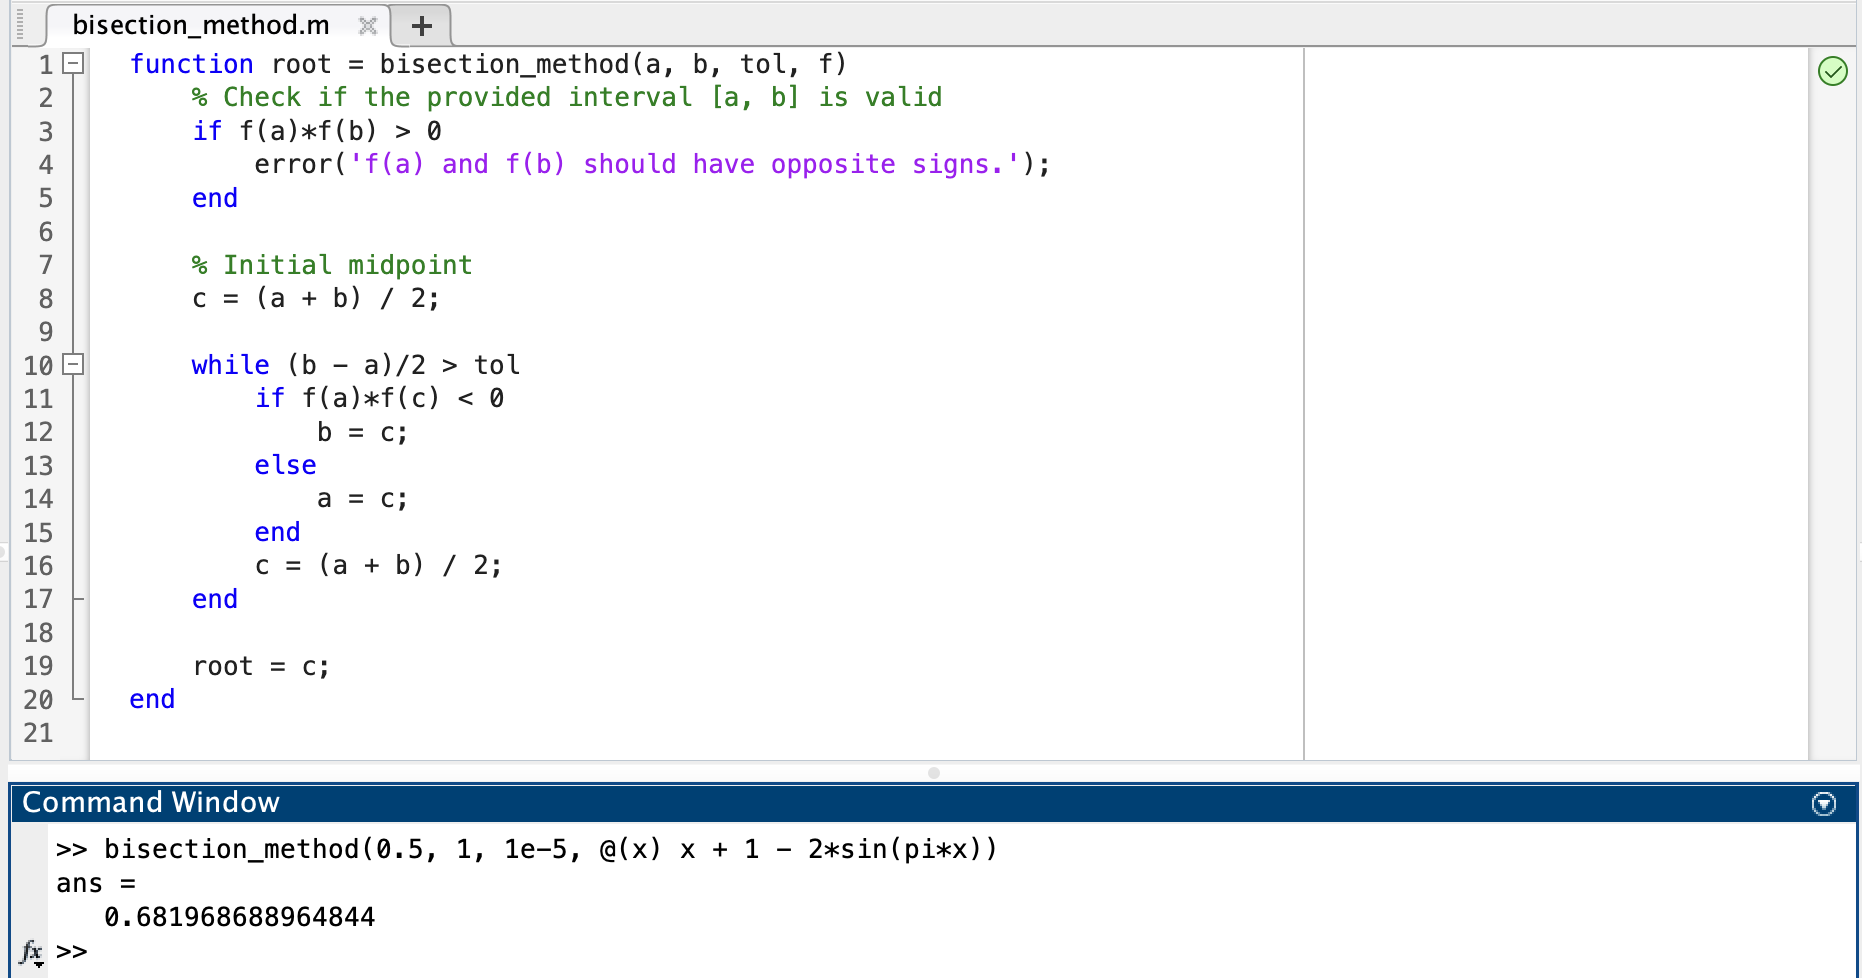
\includegraphics[scale=0.2]{second.png}}
        \qquad\qquad\emph{$0.5\le x\le 1$}\label{fig:2}
    \end{minipage}        
\end{figure} 

\subsection*{Problem 8}
\begin{enumerate}[label=\alph*.]
    \item Sketch the graphs of $y=x$ and $y=tan(x)$.
    \begin{proof}[Solution]\indent 
        \begin{figure}[htb!]
            \centering
            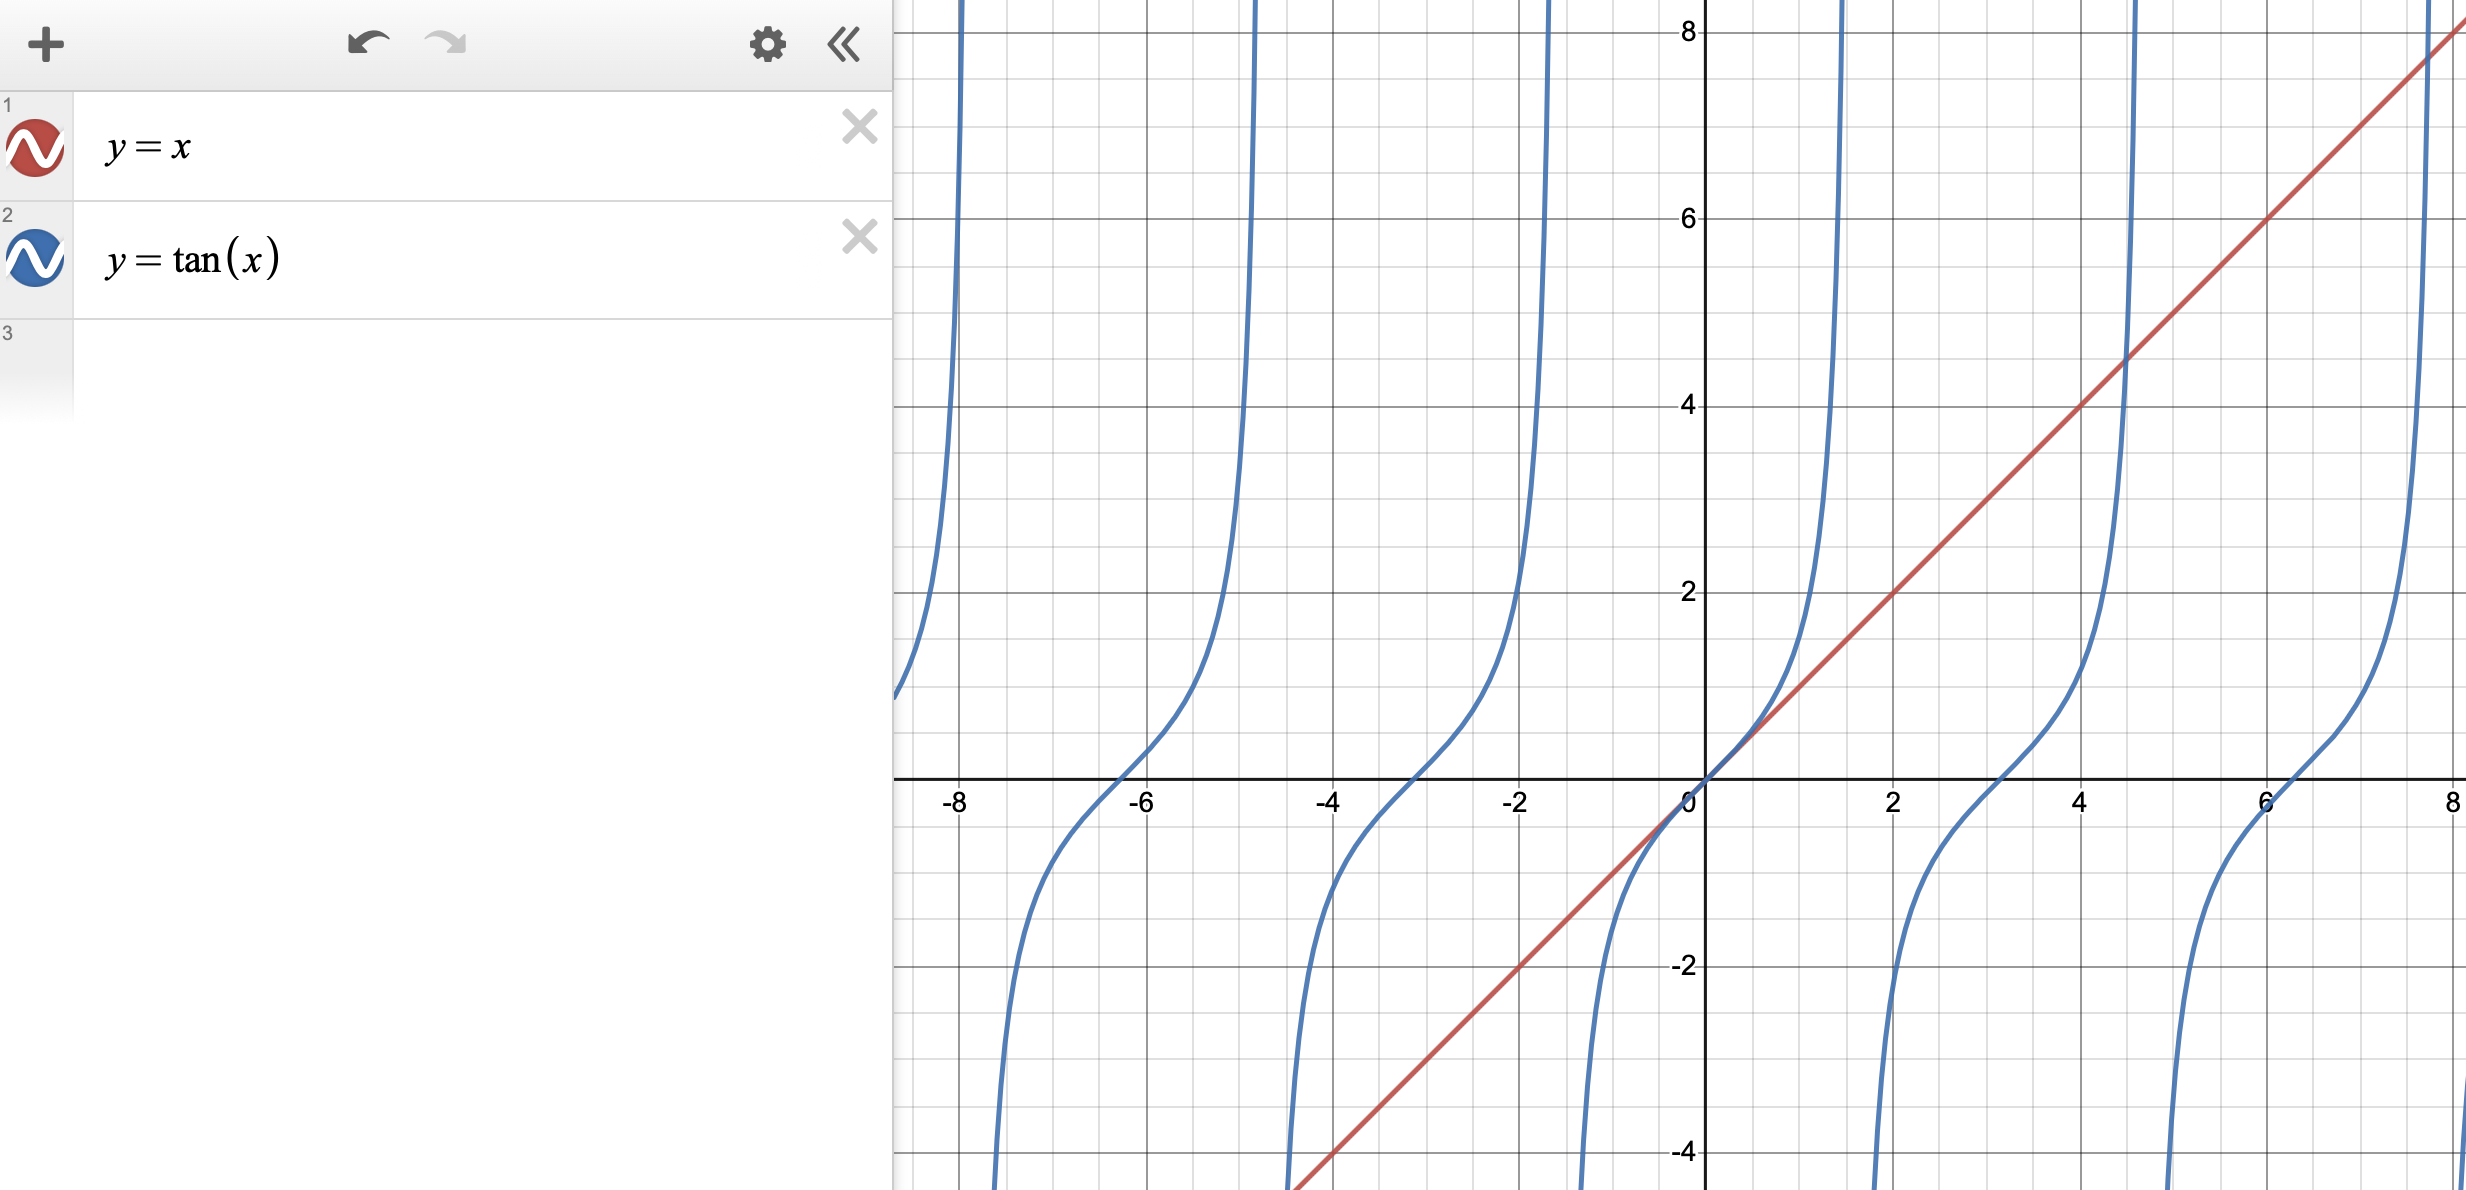
\includegraphics[scale=0.25]{sketch.png}
            \caption{Too trivial to draw by hand.}
        \end{figure}
    \end{proof}
    
    \newpage
    \item Use the Bisection method to find an approximation to within $10^{-5}$ to the first positive 
    value of $x$ with $x = tan(x)$.
    \begin{proof}[Solution]
        We use the same function coded from last problem to solve the equation $tan(x) - x = 0$ on 
        the interval $[4, 4.6]$.
        \begin{figure}[htb!]
            \centering
            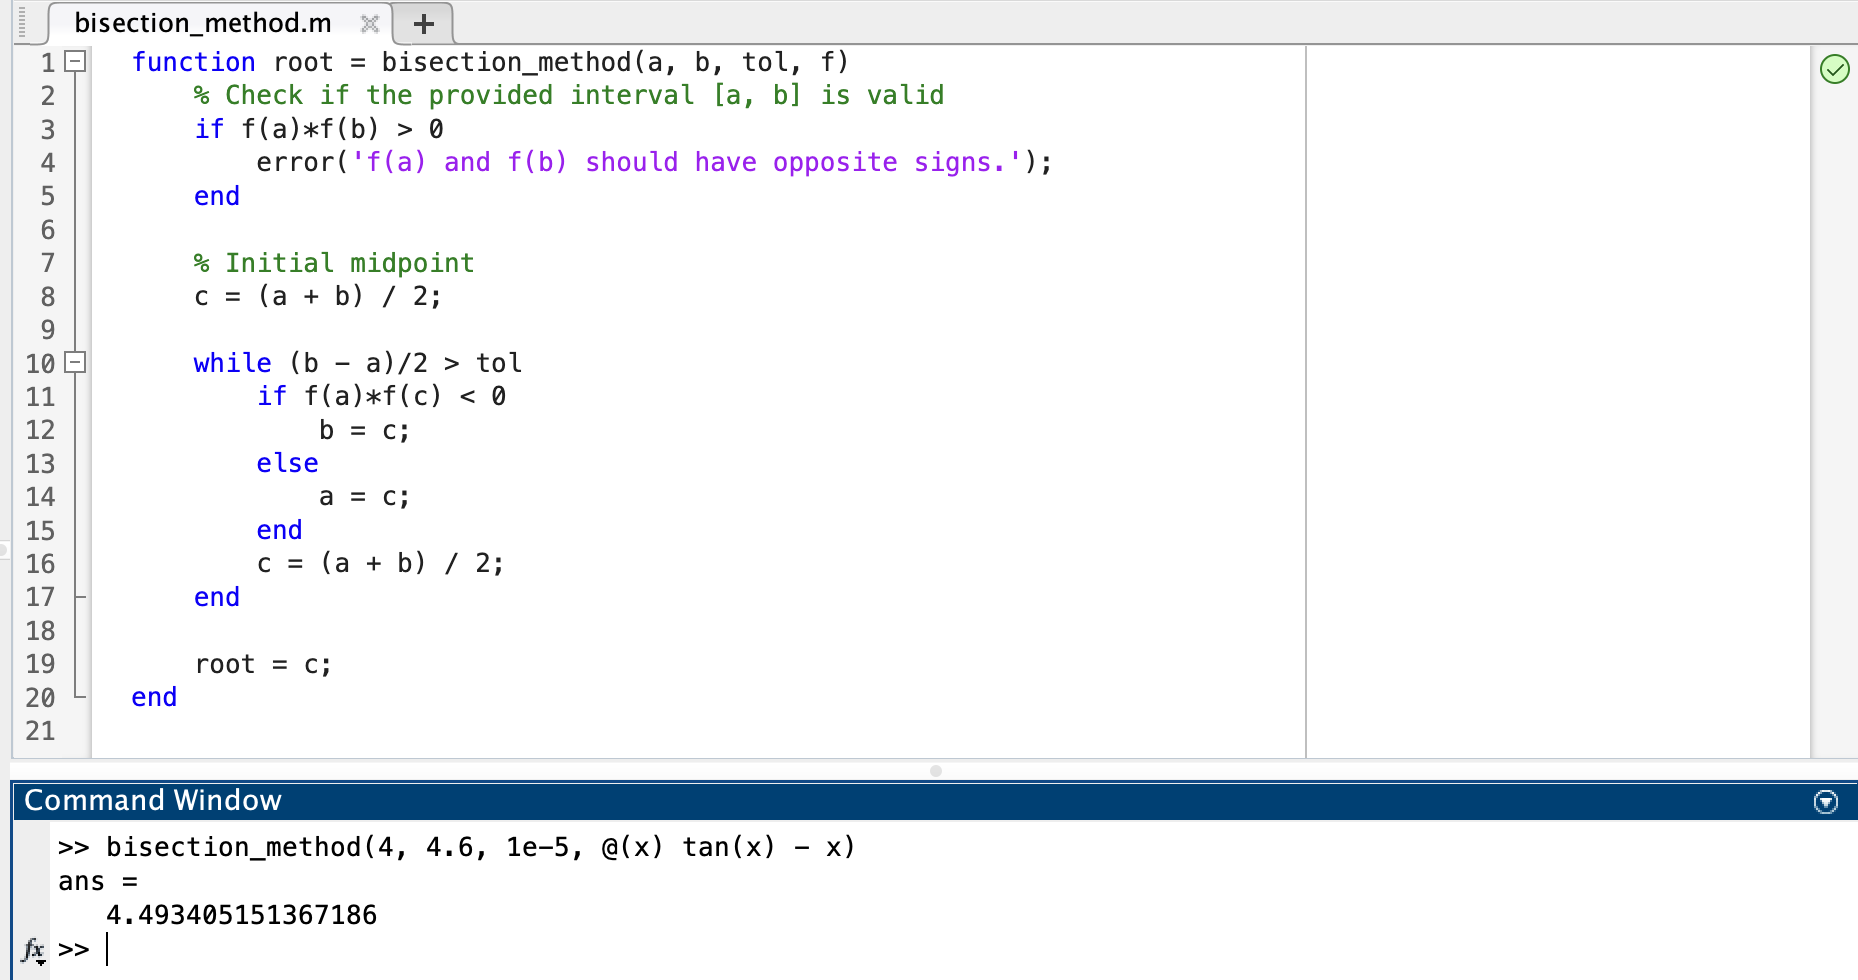
\includegraphics[scale=0.25]{8b.png}
        \end{figure}
    \end{proof}
\end{enumerate}

\subsection*{Problem 20}
Let $f(x) = (x-1)^{10}, p=1$, and $p_n = 1+\frac{1}{n}$. Show that $|f(p_n)|<10^{-3}$ whenever $n>1$ 
but that $|p-p_n|<10^{-3}$ requires that $n>1000$.

\begin{proof}
    $f(p_n) = (1+\frac{1}{n}-1)^{10} = \left(\frac{1}{n}\right)^{10}$. Notice that 
    $\left(\frac{1}{n}\right)^{10}$ is a positive function. Then $|f(p_n)| = \frac{1}{n^{10}} < 
    10^{-3} \Rightarrow n > \sqrt[10]{1000} \Rightarrow n > 1.996 \Rightarrow n > 1$ for $n \in 
    \mathbb{N}$.

    Notice $p_n > p$ for all $n$. Hence, $|p-p_n| = p_n - p = \frac{1}{n}$. Then, we have 
    $\frac{1}{n} < 10^{-3} \Rightarrow n > 1000$.
\end{proof}

\end{document}
